% =============================================
% =============================================
% Document class: Article
\documentclass[ a4paper, twoside, 11pt]{article}
% Packages: LaTeX (Depth-1)
\usepackage[ vlined, linesnumbered, ruled]{algorithm2e}
\usepackage{ amsfonts, amsmath, amssymb, amsthm}
\usepackage[ titletoc, title]{appendix}
\usepackage{ bbm}
\usepackage{ color}
\usepackage{ dsfont}
\usepackage{ enumitem}
\usepackage{ graphicx}
\usepackage{ fancyhdr, float, fullpage}
\usepackage{ hyperref}
\usepackage{ lastpage, latexsym, lipsum}
\usepackage{ mathrsfs, mathtools, multicol}
\usepackage{ parskip}
\usepackage{ setspace, stmaryrd, subcaption}
\usepackage{ tabularx}
\usepackage{ wasysym}
\usepackage[ dvipsnames, table]{ xcolor}
\usepackage{ xfrac}
% Packages: LaTeX (Depth-2)
\usepackage{ epstopdf}

% =============================================
\topmargin 			= -1.6cm
\headheight 		= .90cm
\headsep 			= .80cm
\textheight 		= 24.0cm
\textwidth 			= 15.5cm
\oddsidemargin		= 0.cm
\evensidemargin 	= 0.cm

% =============================================
% =============================================
% Macros: Language
\newcommand{\define}{\triangleq}
\newcommand{\done}{\hfill $\square$}
%\newcommand{\eqCIRC}{\stackrel{\circ}{=}}
%\newcommand{\eqSTAR}{\stackrel{*}{=}}
\renewcommand{\epsilon}{\varepsilon}
\newcommand{\eg}{\textit{e.g.,\;}}
\newcommand{\egc}{\textit{e.g.:\;}}
\newcommand{\Eg}{\textit{E.g.,\;}}
\newcommand{\Egc}{\textit{E.g.:\;}}
\newcommand{\ie}{\textit{i.e.,\;}}
\newcommand{\iec}{\textit{i.e.:\;}}
\newcommand{\Ie}{\textit{I.e.,\;}}
\newcommand{\Iec}{\textit{I.e.:\;}}
\newcommand{\QED}{\hfill $\blacksquare$}
\renewcommand{\tilde}[1]{\widetilde{#1}}
\newcommand{\tsup}[1]{\ensuremath{^{\text{#1}}}}
\newcommand{\tsub}[1]{\ensuremath{_{\text{#1}}}}
\renewcommand{\vec}[1]{{\boldsymbol{#1}}}

% Macros: Optimization & Probability
\DeclareMathOperator*{\argmax}{arg\,max}
\DeclareMathOperator*{\argmin}{arg\,min}
\newcommand{\Exp}{\mathbb{E}}
\newcommand{\Indicate}[1]{ \IndFun \, \{ \, #1 \, \} }
\renewcommand{\Pr}{\mathbb{P}}
\newcommand{\Normal}{\mathcal{N}}
\newcommand{\std}{\text{std}}
\newcommand{\var}{\text{var}}

% Macros: Sets
\newcommand{\Complex}{\mathbb{C}}
\renewcommand{\emptyset}{\varnothing}
\newcommand{\Nat}{\mathbb{N}}
\renewcommand{\Re}{\mathbb{R}}
\newcommand{\ReNN}{{\Re}_{\geq 0}}
\newcommand{\ReSP}{{\Re}_{> 0}}
\renewcommand{\subset}{\subseteq}
\renewcommand{\supset}{\supseteq}
\newcommand{\Z}{\mathbb{Z}}
\newcommand{\ZNN}{{\Z}_{\geq 0}}

% Macros: Spacing & Other Commands
\newcommand{\fullcut}{\vspace{-\baselineskip}}
\newcommand{\fullskip}{\vspace{\baselineskip}}
\newcommand{\halfcut}{\vspace{-0.5\baselineskip}}
\newcommand{\halfskip}{\vspace{0.5\baselineskip}}
\renewcommand{\figurename}{Figura}
\renewcommand{\tablename}{Tabla}

% =============================================
% Sesion de Clase
\newcommand{\sesion}{02}
% Macros para definiciones, teoremas, etc
\newcounter{sesion}
\setcounter{sesion}{\sesion}
\theoremstyle{definition}
\newtheorem{definition}{Definici\'on}[sesion]
\newtheorem{example}[definition]{Ejemplo}
\newtheorem{exercise}[definition]{Ejercicio}
\newtheorem{note}[definition]{Nota}
\newtheorem{problem}[definition]{Problema}
\newtheorem{theorem}[definition]{Teorema}

% =============================================
% =============================================
\newcommand{\HeaderLine}{}
\newcommand{\FooterLine}{P\'agina \thepage ~de \pageref*{LastPage}}

\pagestyle{fancyplain}
\fancyhf{}

\rhead[]{\fancyplain{}{\HeaderLine}}
\lhead[\fancyplain{}{\HeaderLine}]{}
\lfoot[\fancyplain{}{\FooterLine}]{}
\rfoot[]{\fancyplain{}{\FooterLine}}

\renewcommand{\headrulewidth}{0.4pt}
\renewcommand{\footrulewidth}{0.4pt}
\renewcommand{\thefootnote}{\fnsymbol{footnote}}

% =============================================
% =============================================
\begin{document}
\allowdisplaybreaks

\begin{center}
\Large Din\'amica (FIMCP-01271): Lecci\'on \sesion \\[0.5ex]
\small \textbf{A\~no:} 2016-2017 \qquad \textbf{T\'ermino:} II \qquad
\textbf{Instructor:} Luis I. Reyes Castro \qquad \textbf{Paralelo:} 02
\end{center}
\halfskip

\fbox{

\begin{minipage}[b][\height][t]{\textwidth}
\vspace{0.2 cm}

\begin{center}
\textbf{COMPROMISO DE HONOR}
\end{center}
\vspace{0.4 cm}

\scriptsize
{
Yo, \rule{60mm}{.1pt} al firmar este compromiso, reconozco que la presente lecci\'on est\'a dise\~nada para ser resuelta de manera individual, que puedo usar un l\'apiz o pluma y una calculadora cient\'ifica, \linebreak que solo puedo comunicarme con la persona responsable de la recepci\'on de la lecci\'on, y que cualquier instrumento de comunicaci\'on que hubiere tra\'ido debo apagarlo. Tambi\'en estoy conciente que no debo consultar libros, notas, \linebreak ni materiales did\'acticos adicionales a los que el instructor entregue durante la lecci\'on o autorice a utilizar. Finalmente, me comprometo a desarrollar y presentar mis respuestas de manera clara y ordenada. \\

Firmo al pie del presente compromiso como constancia de haberlo le\'ido y aceptado. 
\vspace{0.4 cm}

Firma: \rule{60mm}{.1pt} \qquad N\'umero de matr\'icula: \rule{40mm}{.1pt} \hspace{0.5cm} \\[-0.8ex]

}

\end{minipage}

}
\fullskip

% =============================================
\begin{problem}
En la figura de abajo, el bloque $A$ se mueve hacia abajo con una velocidad constante de 75 mm/s, mientras que el bloque $C$ inicia su movimiento desde el reposo en $t = 0$ y se mueve hacia arriba con una aceleraci\'on constante de 25 mm/s\tsup{2}. Adem\'as, el punto $D$ \linebreak indica la polea a la cual est\'a fijado el extremo derecho de la cuerda del lado izquierdo. Tomando como origen el techo y como direcci\'on positiva la direcci\'on hacia abajo, encuentre: 
\begin{figure}[htb]
\centering
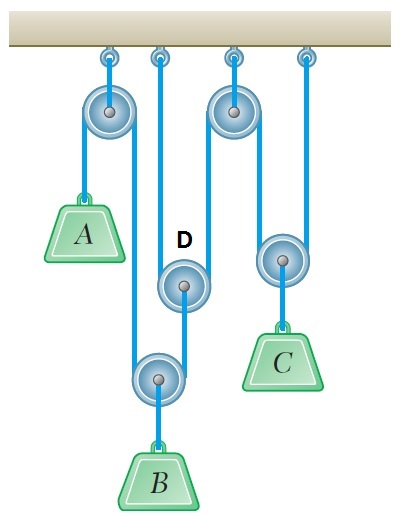
\includegraphics[ width = 0.30\textwidth]{fig_P11-186.jpg}
\end{figure}

\begin{enumerate}[label=\alph*.]
\item \textbf{[2 Puntos]} Las longitudes de las dos cuerdas como funciones de las posiciones de los bloques $A$, $B$ y $C$ y del punto $D$. Den\'otese a la longitud de la cuerda del lado izquierdo como $\ell_1$ y a la del lado derecho como $\ell_2$. \\ \emph{Soluci\'on:} De la figura vemos que: 
\begin{align*}
\ell_1 \; 
& = \; x_A(t) + x_B(t) + ( \, x_B(t) - x_D(t) \, ) 
\; = \; x_A + 2 \, x_B(t) - x_D(t) \\
\ell_2 \; & = \; 2 \, x_C(t) + 2 \, x_D(t)
\end{align*}
\item \textbf{[2 Puntos]} Una ecuaci\'on que relacione las velocidades de los bloques $A$, $B$ y $C$. \\ \emph{Soluci\'on:} Primero diferenciamos las dos ecuaciones anteriores con respecto al tiempo, para obtener: 
\begin{align*}
0 \; 
& = \; v_A(t) + 2 \, v_B(t) - v_D(t) \\
0 \; & = \; 2 \, v_C(t) + 2 \, v_D(t)
\end{align*}
Luego, reconocemos que la segunda ecuaci\'on dice que $v_D(t) = -v_C(t)$. Reemplazando esto en la primera ecuaci\'on, tenemos: 
\[
v_A(t) + 2 \, v_B(t) + v_C(t) \; = \; 0
\]
\item \textbf{[1 Punto]} El tiempo transcurrido hasta que la velocidad del bloque $B$ sea cero. \\ \emph{Soluci\'on:} Resolviendo la ecuaci\'on anterior para $v_B(t)$ obtenemos: 
\[
v_B(t) \; = \; -(1/2)( \, v_A(t) + v_C(t) \, )
\]
Como $v_A(t) = 75$ mm/s, y como $v_C(t) = -25 \, t$ mm/s, tenemos: 
\[
v_B(t) \; = \; -(1/2)( \, 75 - 25 \, t \, )
\]
Vemos asi que $v_B(t) = 0$ cuando $t = 3$ s. 
\item \textbf{[1 Punto]} El desplazamiento del bloque $B$. \\ \emph{Soluci\'on:} Recordando que conocemos $v_B(t)$ para todo $t$, vemos que: 
\begin{align*}
\Delta x 
\; = \; \int_0^3 v_B(t) \, dt \; 
& = \; - \frac{1}{2} \, 
\int_0^3 ( \, 75 - 25 \, t \, ) \, dt \\[1ex]
& = \; - \frac{1}{2} \, 
\left[ \, 75 \, t + \frac{25}{2} \, t^2 \, \right]_0^3 \\[1ex]
& = \; -\frac{225}{4} \text{ mm} \; = \; -56.25 \text{ mm}
\end{align*}
\end{enumerate}

\end{problem}
\vspace{\baselineskip}

% =============================================
\begin{problem}
En la figura de abajo, los tres bloques mostrados se mueven a velocidades constantes. Si se sabe que la velocidad relativa de $A$ con respecto a $C$ es de 300 mm/s hacia arriba, y que la velocidad relativa de $B$ con respecto a $A$ es de 200 mm/s hacia abajo, encuentre: 
\begin{figure}[H]
\centering
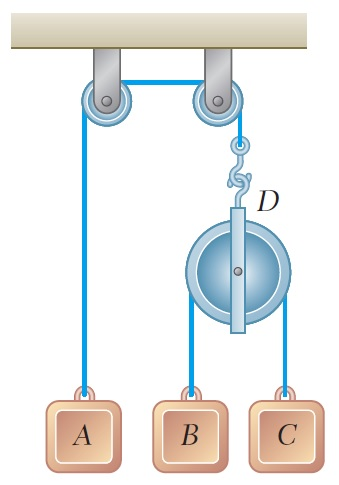
\includegraphics[ width = 0.25\textwidth]{fig_P11-187.jpg}
\end{figure}

\begin{enumerate}[label=\alph*.]
\item \textbf{[1 Punto]} Una ecuaci\'on que relacione la velocidad del bloque $A$ con la velocidad del punto $D$. \\ \emph{Soluci\'on:} Es f\'acil ver que $v_D(t) = - v_A(t)$. 
\item \textbf{[1 Punto]} Una ecuaci\'on que relacione las velocidades de los bloques $B$ y $C$ con la velocidad del punto $D$. \\ \emph{Soluci\'on:} Si denotamos a la longitud de la cuerda que une a los bloques $B$ y $C$ con el punto $D$ como $\ell$, vemos que: 
\[
\ell 
\; = \; ( \, x_B(t) - x_D(t) \, ) + ( \, x_C(t) - x_D(t) \, ) 
\; = \; x_B(t) + x_C(t) - 2 \, x_D(t)
\]
Diferenciando esta ecuaci\'on, obtenemos la relaci\'on deseada: 
\[
v_B(t) + v_C(t) - 2 \, v_D(t) \; = \; 0
\]
\item \textbf{[1 Punto]} Un conjunto de tres ecuaciones lineales que relacione las velocidades de los tres bloques. \\ \emph{Soluci\'on:} Las dos primeras dos ecuaciones son obtenidas directamente del enunciado del problema. Ciertamente: 
\begin{itemize}
\item Como $v_{A/C} = -300$ mm/s tenemos: 
\[
v_A(t) - v_C(t) \; = \; -300
\]
\item Como $v_{B/A} = 200$ mm/s tenemos:
\[
v_B(t) - v_A(t) \; = \; 200
\]
\end{itemize}
La \'ultima ecuaci\'on se obtiene al combinar las ecuaciones solicitadas en los dos primeros literales. En particular, como $v_D(t) = - v_A(t)$ y $v_B(t) + v_C(t) - 2 \, v_D(t) = 0$ tenemos: 
\[
2 \, v_A(t) + v_B(t) + v_C(t) \; = \; 0
\]
\item \textbf{[1 Punto]} La velocidad de cada uno de los tres bloques. \\ \emph{Soluci\'on:} Resolviendo las tres ecuaciones lineales obtenemos: 
\[
v_A(t) \; = \; -125 \text{ mm/s} \qquad \qquad
v_B(t) \; = \; +75 \text{ mm/s} \qquad \qquad
v_C(t) \; = \; +175 \text{ mm/s}
\]
\end{enumerate}

\end{problem}
\vspace{\baselineskip}

\end{document}
